% =====================================================================
%  Livrable 1 : question de recherche, collecte, description du dataset,
%  prétraitement. Chiffres issus du code de la branche main
%  (manifestes/niveau2_2026-10-26.json).
% =====================================================================

\section{Question de recherche}

Depuis 2021, les pénuries de médicaments se multiplient en Europe. Les agences sanitaires publient chaque jour la
liste des pénuries en cours, mais personne ne cherche à les \emph{anticiper}. Notre question principale :

\begin{quote}
\textbf{Peut-on prévoir qu'une substance active va manquer en France, et pourquoi ?}
\end{quote}

Deux questions en découlent. \textbf{Les pénuries se propagent-elles} d'un médicament à ses substituts, vers lesquels
les prescriptions se reportent ? \textbf{Sont-elles importées}, c'est-à-dire annoncées par une pénurie de la même
substance en Italie ou en Allemagne ? Nous travaillons sur la France parce que c'est le seul pays pour lequel nous
disposons de la liste complète des médicaments commercialisés, y compris ceux qui ne manquent jamais : sans eux,
impossible d'apprendre ce qui distingue une substance fragile d'une substance robuste.

\section{Collecte et construction du dataset}

\textbf{Les sources.} Toutes les données sont officielles et publiques :
\begin{itemize}
  \item \textbf{ANSM} (agence française) : la page publique des pénuries, et les signalements de rupture que les
  laboratoires doivent lui déclarer, publiés chaque année depuis 2019 ;
  \item \textbf{BDPM} (base publique du médicament) : tous les médicaments vendus en France ;
  \item \textbf{Open Medic} (Assurance Maladie) : les boîtes remboursées par an et la classification ATC des substances ;
  \item \textbf{AIFA} et \textbf{BfArM} : les listes de pénuries italienne et allemande.
\end{itemize}
Ces listes ne montrent que le \emph{présent} : une pénurie terminée disparaît. Pour reconstruire le passé, nous avons
récupéré les \textbf{archives mensuelles de la Wayback Machine}, une photo de chaque liste par mois depuis 2021 (2024
pour l'Allemagne, 2015 pour la base des médicaments).

\textbf{Une construction en trois niveaux}, comme un entrepôt de données (cours \emph{Building a Dataset from a
Warehouse}, TP MegaStore) :

\begin{center}
\begin{tikzpicture}[
  niveau/.style={rounded corners=6pt, fill=#1!9, draw=#1!35, line width=0.6pt, align=center, font=\small,
                 text width=5.0cm, minimum height=1.6cm, inner sep=5pt,
                 execute at begin node={\hyphenpenalty=10000\exhyphenpenalty=10000},
                 drop shadow={opacity=0.12, shadow xshift=0.6pt, shadow yshift=-0.8pt}},
  titre/.style={fill=#1, text=white, font=\footnotesize\bfseries, rounded corners=3pt, inner xsep=6pt,
                inner ysep=2.5pt, text height=1.9ex, text depth=0.5ex, anchor=south west},
  fleche/.style={-{Latex[length=5pt, width=6pt]}, line width=1.4pt, gray!45}]
\node[niveau=niveaubrut] (brut) {272 fichiers sources, gardés tels quels et tracés (adresse, date, empreinte)};
\node[niveau=niveaupropre, right=0.5cm of brut] (propre) {22 tables en schéma en étoile : les épisodes et leurs
  dimensions};
\node[niveau=niveaufinal, right=0.5cm of propre] (final) {une ligne par substance et par mois : variables avant,
  cible après};
\node[titre=niveaubrut] at ([xshift=6pt, yshift=2pt]brut.north west) {1 \enspace BRUT};
\node[titre=niveaupropre] at ([xshift=6pt, yshift=2pt]propre.north west) {2 \enspace NETTOYÉ};
\node[titre=niveaufinal] at ([xshift=6pt, yshift=2pt]final.north west) {3 \enspace FINAL \textmd{(à venir)}};
\draw[fleche] (brut) -- (propre);
\draw[fleche] (propre) -- (final);
\end{tikzpicture}
\end{center}

Trois éléments du cours y sont appliqués :
\begin{itemize}
  \item le \textbf{sens d'une ligne} (grain) de chaque table est écrit et vérifié ;
  \item la base des médicaments est \textbf{historisée} (une version par période, jointure \emph{as-of}), pour décrire
  le marché tel qu'il était à chaque date ;
  \item chaque construction est \textbf{contrôlée et tracée} : aucune ligne perdue ni dupliquée, et un manifeste dit si
  un écart vient du code ou des données.
\end{itemize}

\section{Le dataset}

Le tableau~\ref{tab:tables} donne le nombre d'observations des principales tables, et le tableau~\ref{tab:variables} le sens
des variables d'un épisode de pénurie. Les \textbf{signalements} français serviront de cible à la prédiction.

\begin{table}[H]
\centering\small
\renewcommand{\arraystretch}{1.25}
\rowcolors{2}{white}{niveaubrut!6}
\begin{tabular}{l l r l}
\rowcolor{niveaubrut!16}
\entete{Table} & \entete{Une ligne =} & \entete{Lignes} & \entete{Période} \\
Épisodes, France & une pénurie publiée par l'ANSM & 1\,599 & 2021--2026 \\
Épisodes, Italie & une pénurie publiée par l'AIFA & 10\,035 & 2021--2026 \\
Épisodes, Allemagne & une pénurie publiée par le BfArM & 2\,000 & 2024--2026 \\
Signalements, France & une déclaration d'un laboratoire à l'ANSM & 22\,501 & 2019--2025 \\
Médicaments, France & un médicament commercialisé & 13\,650 & 2026 \\
\filet
\end{tabular}
\caption{Les principales tables et leur nombre d'observations.}
\label{tab:tables}
\end{table}

\begin{table}[H]
\centering\small
\renewcommand{\arraystretch}{1.25}
\rowcolors{2}{white}{niveaubrut!6}
\begin{tabularx}{\linewidth}{l X}
\rowcolor{niveaubrut!16}
\entete{Variable} & \entete{Signification} \\
\texttt{\color{niveaubrut!30!black}atc5} & la substance active (code ATC niveau 5) : la clé qui relie les pays entre eux \\
\texttt{\color{niveaubrut!30!black}atc4} & la classe thérapeutique : les substances d'une même classe sont des substituts \\
\texttt{\color{niveaubrut!30!black}debut}, \texttt{\color{niveaubrut!30!black}fin} & le début et la fin de la pénurie \\
\texttt{\color{niveaubrut!30!black}publication} & la date à laquelle la pénurie apparaît sur la liste, c'est-à-dire devient connue \\
\texttt{\color{niveaubrut!30!black}gravite} & en France : risque de rupture, tension ou rupture \\
\texttt{\color{niveaubrut!30!black}raison} & en Italie et en Allemagne : la cause déclarée (production, forte demande…) \\
\filet
\end{tabularx}
\caption{Les variables principales d'un épisode de pénurie.}
\label{tab:variables}
\end{table}

\begin{figure}[H]
\centering
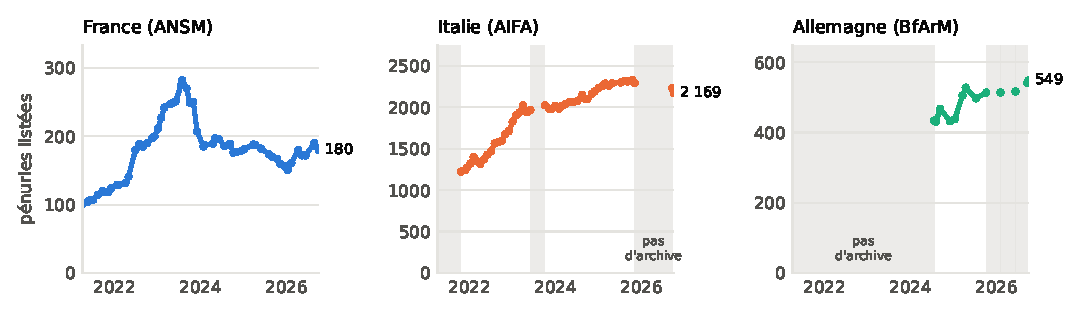
\includegraphics[width=0.74\linewidth]{figures/evolution_penuries.pdf}
\caption{Nombre de pénuries en cours sur chaque archive mensuelle. Zones grises : mois sans archive.}
\label{fig:evolution}
\end{figure}

Trois constats ressortent déjà (figure~\ref{fig:evolution}) :
\begin{itemize}
  \item en France, les pénuries culminent pendant l'hiver 2022-2023, au moment de la crise des antibiotiques ; une
  pénurie dure en général environ \textbf{4 mois}, et près d'une sur cinq plus d'un an ;
  \item \textbf{un tiers des substances} vendues en France a connu au moins une pénurie depuis 2021 ;
  \item près de \textbf{trois substances françaises en pénurie sur quatre} l'ont aussi été en Italie ou en Allemagne,
  ce qui rend la question des pénuries importées pertinente.
\end{itemize}

\section{Prétraitement et choix}

\textbf{Relier les sources entre elles.} Ni l'ANSM ni la BDPM n'indiquent la substance sous forme de code. Nous
la retrouvons en croisant les sources (boîte, nom, substance) : 9 lignes sur 10 sont reliées.

\textbf{Passer des photos aux épisodes.} Une archive mensuelle n'est qu'une photo. Nous regroupons les photos
successives d'un même médicament en un épisode, avec une date de début et une date de fin.

\textbf{Ne jamais utiliser le futur.} Pour prédire, on ne doit utiliser que ce qui était connu au moment de la
prédiction. Nous gardons donc la date de \texttt{publication} d'une pénurie à côté de sa date de début : le début
déclaré est parfois connu après coup, ou annoncé à l'avance.

\textbf{Écarter ce qui fausserait les données.} Les arrêts définitifs de commercialisation ne sont pas des pénuries,
et certaines archives ont été tronquées par la Wayback Machine : les deux sont exclus.

\textbf{Limites.} Les signalements ne concernent que les médicaments jugés essentiels, et les pays ne définissent pas
une pénurie de la même façon : ces différences seront prises en compte dans l'analyse.
